%%%%%%%%%%%%%%%%%%%%%%%%%%%%%%%%%%%%%%%%%%%%%%%%%%%%%%%%%%%%%%%%%%%%%%%%%%%%%%%%%
%%% Capa da prova
\begin{coverpages}

\begin{center}
\textbf{\Large%
Introdução à Ciência da Computação\\
--- 1ª Avaliação ---}
\end{center}

\vspace{0.6cm}

\begin{center}
\textbf{Odisseia}, de Homero.

\vspace{0.5cm}
Excerto do Canto XII:
\end{center}
\vspace{0.3cm}
\small{%
\begin{wrapfigure}{R}{0.4  \textwidth}
\vspace{-1cm}
\begin{center}
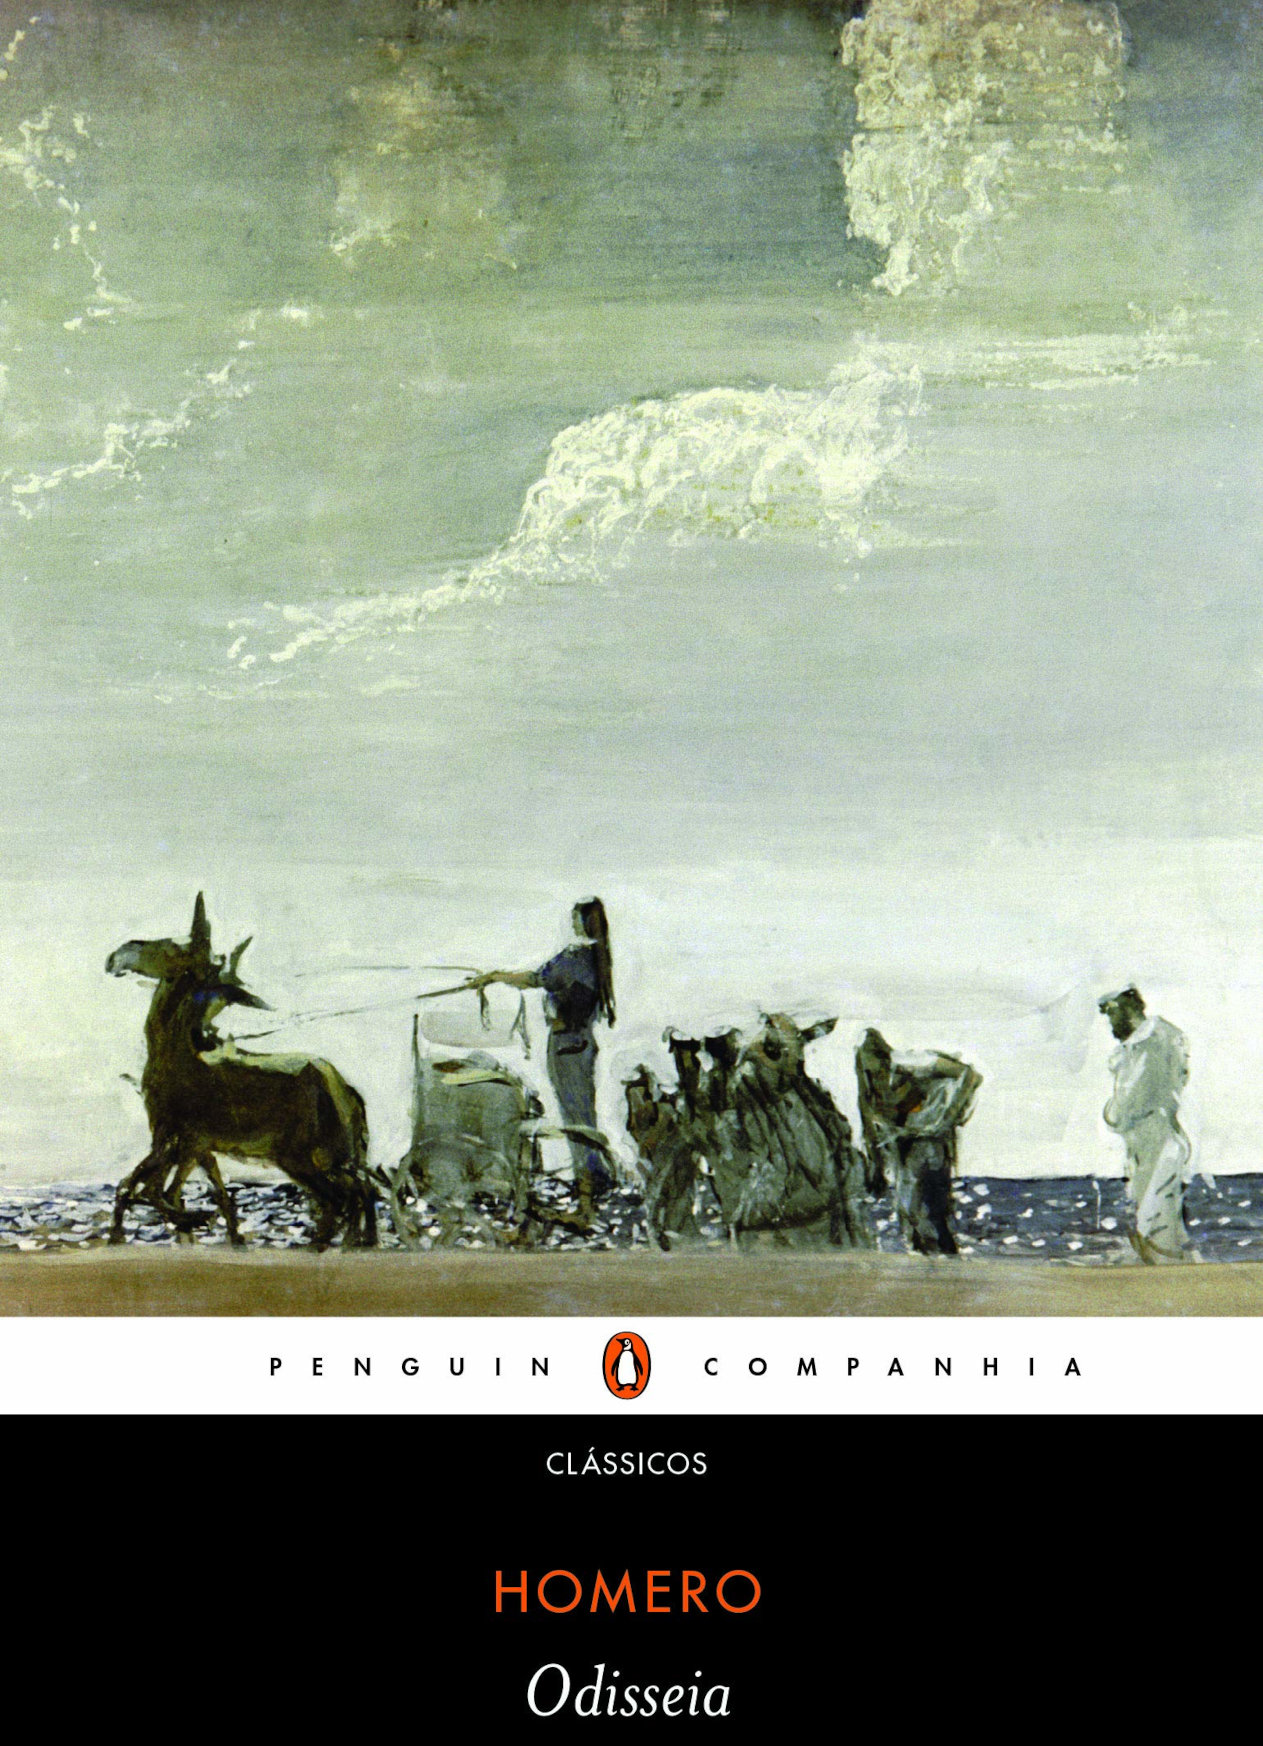
\includegraphics[scale=0.53]{imagens/cover/odisseia2.jpg}\\
\footnotesize{Odisseia, de Homero.\\
Tradução de Frederico Lourenço, publicada\\
pela Companhia das Letras, em 2020.}
\vspace{-0.3cm}
\end{center}
\end{wrapfigure}
``Quando a nau deixou a corrente do rio Oceano, chegou às ondas do mar de amplos
caminhos e à ilha de Eeia, onde da Aurora que cedo desponta estão a morada, os
lugares das suas danças e o nascer do Sol. Foi aí que aportamos, trazendo a nau
para a areia; e nós próprios desembarcamos na praia, onde adormecemos à espera
da Aurora divina.

Quando surgiu a que cedo desponta, a Aurora de róseos dedos, mandei os
companheiros ao palácio de Circe, para de lá trazerem o morto, o falecido
Elpenor. Depressa cortamos achas, lá onde está o promontório derradeiro, e
fizemos o funeral, chorando lágrimas copiosas. Depois que se queimou o morto com
as suas armas, prepramos um túmulo e sobre ele uma lápide; e em cima fixamos o
remo de bom manejo.

Assim nos ocupávamos; mas, vindos do Hades, a Circe não passamos despercebidos:
arranjou-se depressa e veio ao nosso encontro. E com ela vinham  servas trazendo
pão, carne em abundância e frisante vinho tinto. Em pé no meio de nós, assim
falou a divina entre as deusas: `Homens duros, que descestes vivos à mansão de
Hades, homens de dupla morte! Pois os outros só morrem uma vez. Mas agora comei
pão e bebei vinho ao longo desde dia: ao surgir da Aurora, partireis. Da minha
parte, indicar-vos-ei o caminha e cada coisa explicarei, para que devido a
deliberações malfadadas não padeçais com sofrimentos no mar ou em terra'.

Assim falou e consentiram os nossos orgulhosos corações. Durante o resto do dia,
até o pôr do sol, banqueteamo-nos com carne abundante e vinho doce. Quando se
pôs o sol e sobreveio a escuridão, eles deitaram-se junto das amarras da
nau. Mas Circe, levando-me pela mão, sentou-me longe dos queridos companheiros;
deitando-se ao meu lado, tudo quis saber; e eu tudo lhe contei, pela ordem
certa. Depois tais palavras me dirigiu a excelsa Circe:

`Todas estas coisas foram cumpridas; mas ouve agora aquilo que te direi, e um
deus te recordará. Às Sereias chegarás em primeiro lugar, que todos os homens
enfeitiçam, que delas se aproximam. Quem delas se acercar, insciente, e a voz
ouvir das Sereias, ao lado desse homem nunca a mulher e os filhos estarão para
se rogozijarem com o seu regresso; mas as Sereias o enfeitiçam com seu límpido
canto, sentadas num prado, e à sua volta estão amontoadas ossadas de homens
decompostos e suas peles marcescentes. Prossegue caminho, pondo nos ouvidos dos
companheiros cera doce, para que nenhum deles as ouça. Mas se tu próprio
quiseres ouvir o canto, deixa que, na tua nau veloz, te amarrem as mãos e os pés
enquanto estás de pé contra o mastro; e que as cordas sejam atadas ao mastro,
para que te possas deleitar com a voz das duas Sereias. E se a eles ordenares
que te libertem, então que te amarrem com mais cordas ainda.'{''}}

\vspace{1cm}


\begin{center}
\textit{\textbf{\Large%
--- Introdução à Computação e Programação ---\\
\ \\
Abril/2025}}
\newpage
\ \\
\end{center}

%\vspace{1cm}
%\begin{flushright}
%\textbf{Monitor(es):}\\
%\textit{Monitor 1\\
%Monitor 2}
%\end{flushright}

%\begin{center}
%  \fbox{\fbox{\parbox{5.5in}{\centering
%        Answer the questions in the spaces provided on the
%        question sheets. If you run out of room for an answer,
%        continue on the back of the page.}}}
%\end{center}

\end{coverpages}
